%\documentclass[letterpaper, 12pt, parskip=full,DIV=10]{scrartcl}
% The next three lines are temporary, for todo notes, remove after notes are removed
\documentclass[letterpaper, 12pt, parskip=full,]{scrartcl}
\setlength{\marginparwidth}{4.5cm}
\usepackage[top=2.5cm, bottom=2.5cm, left=1.5cm, right=5cm]{geometry}
% Title and Subtitle added in .tex file
\title{Optimal Policies to Battle the Coronavirus ``Infodemic'' Among Social Media Users in Sub-Saharan Africa}
\subtitle{Preanalysis plan}
\author{Molly Offer-Westort, Leah R. Rosenzweig, Susan Athey}
\date{\today}

% USE: %\documentclass[letterpaper, 12pt, parskip=full,]{scrartcl}

\RequirePackage{etex}

% Graphics
\RequirePackage{graphicx}
\RequirePackage{epsfig}
\RequirePackage{psfrag}
\RequirePackage{wrapfig}
\RequirePackage[all]{xy}
\RequirePackage{listings}
\RequirePackage{verbatim} 
\RequirePackage{color} 
% Bold the 'Figure #' in the caption and separate it from the title/caption with a period
% Captions will be left justified
\RequirePackage[aboveskip=1pt,labelfont=bf,labelsep=period,justification=raggedright,singlelinecheck=off]{caption}


% Tables
\RequirePackage{float}
\RequirePackage{rotating}
\RequirePackage{array}
%\RequirePackage{minipage}
\RequirePackage{booktabs,threeparttable}

% Author
\RequirePackage[blocks]{authblk}
\renewcommand\Affilfont{\small}
\setlength{\affilsep}{0em}

\lstset{breaklines=true,basicstyle=\footnotesize\ttfamily}

% Document formatting
%\RequirePackage{fullpage}
\RequirePackage{setspace}
\RequirePackage{mathptmx}
\RequirePackage[hyphens]{url}
\RequirePackage{microtype} 
\RequirePackage[utf8x]{inputenc}
\RequirePackage{enumitem}
\setlist[itemize]{noitemsep, topsep=0pt}
\RequirePackage[colorinlistoftodos, textsize=footnotesize, color=blue!20!white]{todonotes} % adding to-do notes in working file
%\addtokomafont{disposition}{\normalfont\bfseries} % article fonts
%\setkomafont{descriptionlabel}{\normalfont\bfseries} % article fonts

% Bibliography and citation formatting
\RequirePackage[colorlinks=true, citecolor=blue]{hyperref}

\RequirePackage{nameref}
\RequirePackage[round]{natbib} 
\bibliographystyle{chicago}

% Title and Subtitle added in .tex file
%\author{Molly Offer-Westort}
%\date{\today}

\makeatletter %Set \Title reference
\let\Title\@title
\makeatother

\makeatletter %Set \Subtitle reference
\let\Subtitle\@subtitle
\makeatother

\makeatletter %Set \Author reference
\let\Author\@author
\makeatother

% Header and Footer
\RequirePackage{scrlayer-scrpage}
%\ihead{\textbf{\Title} }
%\ohead{\Author}

\RequirePackage{lastpage}
%\cfoot[]{}
%\ofoot[]{\thepage\ of \pageref{LastPage}}
\pagestyle{scrheadings}
%\setkomafont{pageheadfoot}{\small}
\RequirePackage{footnote}
\deffootnote[1.5em]{.5em}{1em}{\textsuperscript{\thefootnotemark}}


% Equation formatting
\RequirePackage{amsmath,amssymb,amsfonts} 
\RequirePackage{amsthm}
\RequirePackage{bbm}
\RequirePackage{array}
\newcommand\numberthis{\addtocounter{equation}{1}\tag{\theequation}}

\newtheorem{theorem}{Theorem}[section]
\newtheorem{lemma}{Lemma}[section]
\newtheorem{prop}{Proposition}[section]
\newtheorem{corollary}{Corollary}[section]
\newtheorem{hypothesis}{Hypothesis}


% Shortcuts
\newcommand{\nn}{\nonumber}

% Define new characters
\def\Var{{\textrm{Var}}\,}
\def\V{{\textrm V}\,}
\def\E{{\textrm E}\,}
\def\arg{{\textrm {arg} }\,}
\def\Cov{{\textrm{Cov} }\,}
\def\Cor{{\textrm{Cor} }\,}
\def\N{{\textrm N}\,}
\def\Supp{{\textrm {Supp} }\,}
\DeclareMathOperator*{\argmin}{arg\,min}
\DeclareMathOperator*{\argmax}{arg\,max}

%--------------------------------------------------------------------------
% Math boldface shortcuts, etc. ----------------------------------
%--------------------------------------------------------------------------
\newcommand{\A}{\mathbf{A}}\newcommand{\B}{\mathbf{B}}\newcommand{\C}{\mathbf{C}}
\newcommand{\D}{\mathbf{D}}\newcommand{\F}{\mathbf{F}}\newcommand{\G}{\mathbf{G}}
\newcommand{\HB}{\mathbf{H}}\newcommand{\I}{\mathbf{I}}\newcommand{\J}{\mathbf{J}}
\newcommand{\K}{\mathbf{K}}\newcommand{\Lb}{\mathbf{L}}\newcommand{\M}{\mathbf{M}}
\newcommand{\NB}{\mathbf{N}}\newcommand{\OB}{\mathbf{O}}\newcommand{\PB}{\mathbf{P}}
\newcommand{\Q}{\mathbf{Q}}\newcommand{\R}{\mathbf{R}}\newcommand{\SB}{\mathbf{S}}
\newcommand{\T}{\mathbf{T}}\newcommand{\U}{\mathbf{U}}%\newcommand{\V}{\mathbf{V}}
\newcommand{\W}{\mathbf{W}}\newcommand{\X}{\mathbf{X}}\newcommand{\Y}{\mathbf{Y}}
\newcommand{\Z}{\mathbf{Z}}

\newcommand{\aB}{\mathbf{a}}\newcommand{\bB}{\mathbf{b}}\newcommand{\cB}{\mathbf{c}}
\newcommand{\dB}{\mathbf{d}}\newcommand{\e}{\mathbf{e}}\newcommand{\f}{\mathbf{f}}
\newcommand{\g}{\mathbf{g}}\newcommand{\h}{\mathbf{h}}\newcommand{\iB}{\mathbf{i}}
\newcommand{\jB}{\mathbf{j}}\newcommand{\kB}{\mathbf{k}}\newcommand{\lB}{\mathbf{l}}
\newcommand{\m}{\mathbf{m}}\newcommand{\n}{\mathbf{n}}\newcommand{\oB}{\mathbf{o}}
\newcommand{\p}{\mathbf{p}}\newcommand{\q}{\mathbf{q}}\newcommand{\rB}{\mathbf{r}}
\newcommand{\s}{\mathbf{s}}\newcommand{\tB}{\mathbf{t}}\newcommand{\uB}{\mathbf{u}}
\newcommand{\vB}{\mathbf{v}}\newcommand{\w}{\mathbf{w}}\newcommand{\x}{\mathbf{x}}
\newcommand{\y}{\mathbf{y}}\newcommand{\z}{\mathbf{z}}

\def\AA{{\mathbb A}}\def\BB{{\mathbb B}}\def\CC{{\mathbb C}}
\def\DD{{\mathbb D}}\def\EE{{\mathbb E}}\def\FF{{\mathbb F}}
\def\GG{{\mathbb G}}\def\HH{{\mathbb H}}\def\II{{\mathbb I}}
\def\JJ{{\mathbb J}}\def\KK{{\mathbb K}}\def\LL{{\mathbb L}}
\def\MM{{\mathbb M}}\def\NN{{\mathbb N}}\def\OO{{\mathbb O}}
\def\PP{{\mathbb P}}\def\QQ{{\mathbb Q}}\def\RR{{\mathbb R}}
\def\SS{{\mathbb S}}\def\TT{{\mathbb T}}\def\UU{{\mathbb U}}
\def\VV{{\mathbb V}}\def\WW{{\mathbb W}}\def\XX{{\mathbb X}}
\def\YY{{\mathbb Y}}\def\ZZ{{\mathbb Z}}

\RequirePackage{euscript}
\let\muchmore= \gg
\let\muchless= \ll
\let\typewriter=\tt  % for turning on the typewriter font
\def\aa{{\EuScript A}}\def\bb{{\EuScript B}}\def\cc{{\EuScript C}}\def\dd{{\EuScript D}}
\def\ee{{\EuScript E}}\def\ff{{\EuScript F}}\def\gg{{\EuScript G}}\def\hh{{\EuScript H}}
\def\ii{{\EuScript I}}\def\jj{{\EuScript J}}\def\kk{{\EuScript K}}\def\ll{{\EuScript L}}
\def\mm{{\EuScript M}}\def\nn{{\EuScript N}}\def\oo{{\EuScript O}}\def\pp{{\EuScript P}}
\def\qq{{\EuScript Q}}\def\rr{{\EuScript R}}\def\ss{{\EuScript S}}\def\tt{{\EuScript T}}
\def\uu{{\EuScript U}}\def\vv{{\EuScript V}}\def\ww{{\EuScript W}}\def\xx{{\EuScript X}}
\def\yy{{\EuScript Y}}\def\zz{{\EuScript Z}}

\newcommand{\Beta}{\boldsymbol{\beta}}
\newcommand{\btheta}{\boldsymbol{\theta}}
\newcommand{\bgamma}{\boldsymbol{\gamma}}
\newcommand{\bpi}{\boldsymbol{\pi}}
\newcommand{\arrowp}{\stackrel{p}{\rightarrow}}
\newcommand{\0}{\mathbf{0}}
\newcommand{\bP}{\mathbf{P}}

\newcommand\independent{\protect\mathpalette{\protect\independenT}{\perp}}
\def\independenT#1#2{\mathrel{\rlap{$#1#2$}\mkern2mu{#1#2}}}


\newcommand{\indep}{\perp\!\!\!\!\perp}

\thispagestyle{plain}



\begin{document}%
\normalsize%
\maketitle%
\tableofcontents%
\clearpage%


\centerline{\textbf{ABSTRACT}}
\begin{abstract}
Alongside the outbreak of Coronavirus, much of the world’s population is also experiencing an “infodemic” -- the spread of myths and hoax cures related to the virus. Covid-19 misinformation is spreading through online media outlets and social media platforms. While many false cures are largely harmless (e.g., drinking lemon water), others have devastating consequences, such as taking chloroquine. As a result, governments struggling to prepare healthcare systems and encourage citizens to comply with best practices also need to tackle misinformation. Building upon the experimental literature on combating fake news, we evaluate the effect of interventions designed to decrease sharing of false COVID-19 cures. Using Facebook advertisements to recruit social media users in Kenya and Nigeria, we deliver our interventions using a Facebook Messenger chatbot, allowing us to observe treatment effects in a realistic setting. Our aim is to find the context-aware intervention policy that will assign individuals the intervention that is most effective for them, based on their covariate profile. Using a contextual adaptive experimental design to sequentially assign treatment probabilities, we are able to learn the optimal contextual policy, and minimize assignment to ineffective or counter-productive interventions within the experiment. Analyzing heterogeneity in treatment effects allows us to learn whether different interventions are more effective for different people, improving our understanding of how to tackle harmful misinformation during an ongoing health crisis. Finally, we bring comparative data to a global problem for which the existing research has largely been limited to the Global North. This pre-analysis plan describes the research design and outlines the key hypotheses that we will evaluate.
\end{abstract}





\section{Motivation and Research Questions}

% motivation
Alongside the outbreak of Coronavirus, much of the world's population is also experiencing an ``infodemic'' -- the spread of myths and hoax cures related to the virus. Covid-19 misinformation is spreading through online media outlets and social media platforms. These falsities range from incorrect information about government action to hoax cures, some of which are largely harmless, such as drinking lemon water, while others can have devastating consequences if adopted, such as taking chloroquine or drinking bleach. As a result, governments struggling to prepare health care systems and encourage citizens to comply with best practices are also struggling to tackle a pandemic of misinformation.

% what we do 
This project evaluates the effect of interventions designed to decrease sharing of false COVID-19 cures. Using Facebook advertisements to recruit social media users in Kenya and Nigeria, we deliver our interventions using a Facebook Messenger chatbot, allowing us to observe treatment effects in a realistic setting. We test interventions targeted at both the respondent level, such as general warnings, as well as headline-level treatments, such as flags and ``false'' tags (treatments are described in Table~\ref{tab:treatments}). 

Using a contextual adaptive experimental design, we sequentially assign treatment probabilities to privilege assignment to the most effective interventions, and minimize assignment to ineffective or counter-productive interventions. Our aim is to learn an optimal contextual policy that will assign individuals the intervention that is most effective for them, conditional on their covariate profile. Exploring heterogeneity in treatment effects allows us to learn whether different interventions are more effective for different people, improving our understanding of how to tackle harmful misinformation during an ongoing health crisis. 

% how we build on existing lit
This work builds on the experimental literature on combating fake news in several important ways. First, we examine several prominent interventions that have proven successful in other studies and in other settings and use an adaptive design to observe the best intervention policy. Second, we bring comparative data to a global problem. Despite the global nature of the ``infodemic,'' much of the existing research is limited to the Global North, particularly the United States \citep{pennycook2020fighting, bursztyn2020misinformation}.\footnote{Two recent exceptions from sub-Saharan Africa include a field experiment in Zimbabwe using Whatsapp messages from a trusted NGO  to counter COVID misinformation \citep{bowles2020center} and a recent survey among traders in Lagos, Nigeria looking at the correlates of belief in COVID-related misinformation \citep{Grossman2020}.} Finally, this pre-analysis plan describes the research design, outlines the key hypotheses that we will evaluate, and details our approach to analysis.




\section{Case Selection}
% Why kenya + Nigeria?

We examine these questions using a study focused on online social media users in two major English-language hubs of online communication in sub-Saharan Africa, Kenya and Nigeria.  Collectively, there are 38 million Facebook users who are 18 years and older from these two countries (as reported on Facebook's advertising platform). Misinformation and fake news are major problems in these countries. AfricaCheck.org, a third party verification site, has offices in both countries and has recently created pages devoted to COVID-19-related misinformation circulating online. From January to March, the number of English-language fact-checks increased by more than 900\% worldwide \citep{brennen2020types}, demonstrating the prevalence of this kind of content and the availability of verified Coronavirus-related information.  Figure \ref{fig:poynter} illustrates the volume of fact checks that appear in \url{poynter.org}'s global Coronavirus facts database, which demonstrates that Kenya and Nigeria are main factcheck sources on the continent. Thus, there is a large database of verified information from which we can draw stimuli for our experiment in these two countries. 

%% LR: I'm looking for citations to demonstrate these are hubs of misinfo - another way to go is that they are major english media sources and other countries in the region often also read news from ky/ng...

\begin{figure}[htb]
\centering
\caption{Map illustrating the volume of fact-checks in \url{poynter.org}'s global coronavirus facts database.}
\label{fig:poynter}
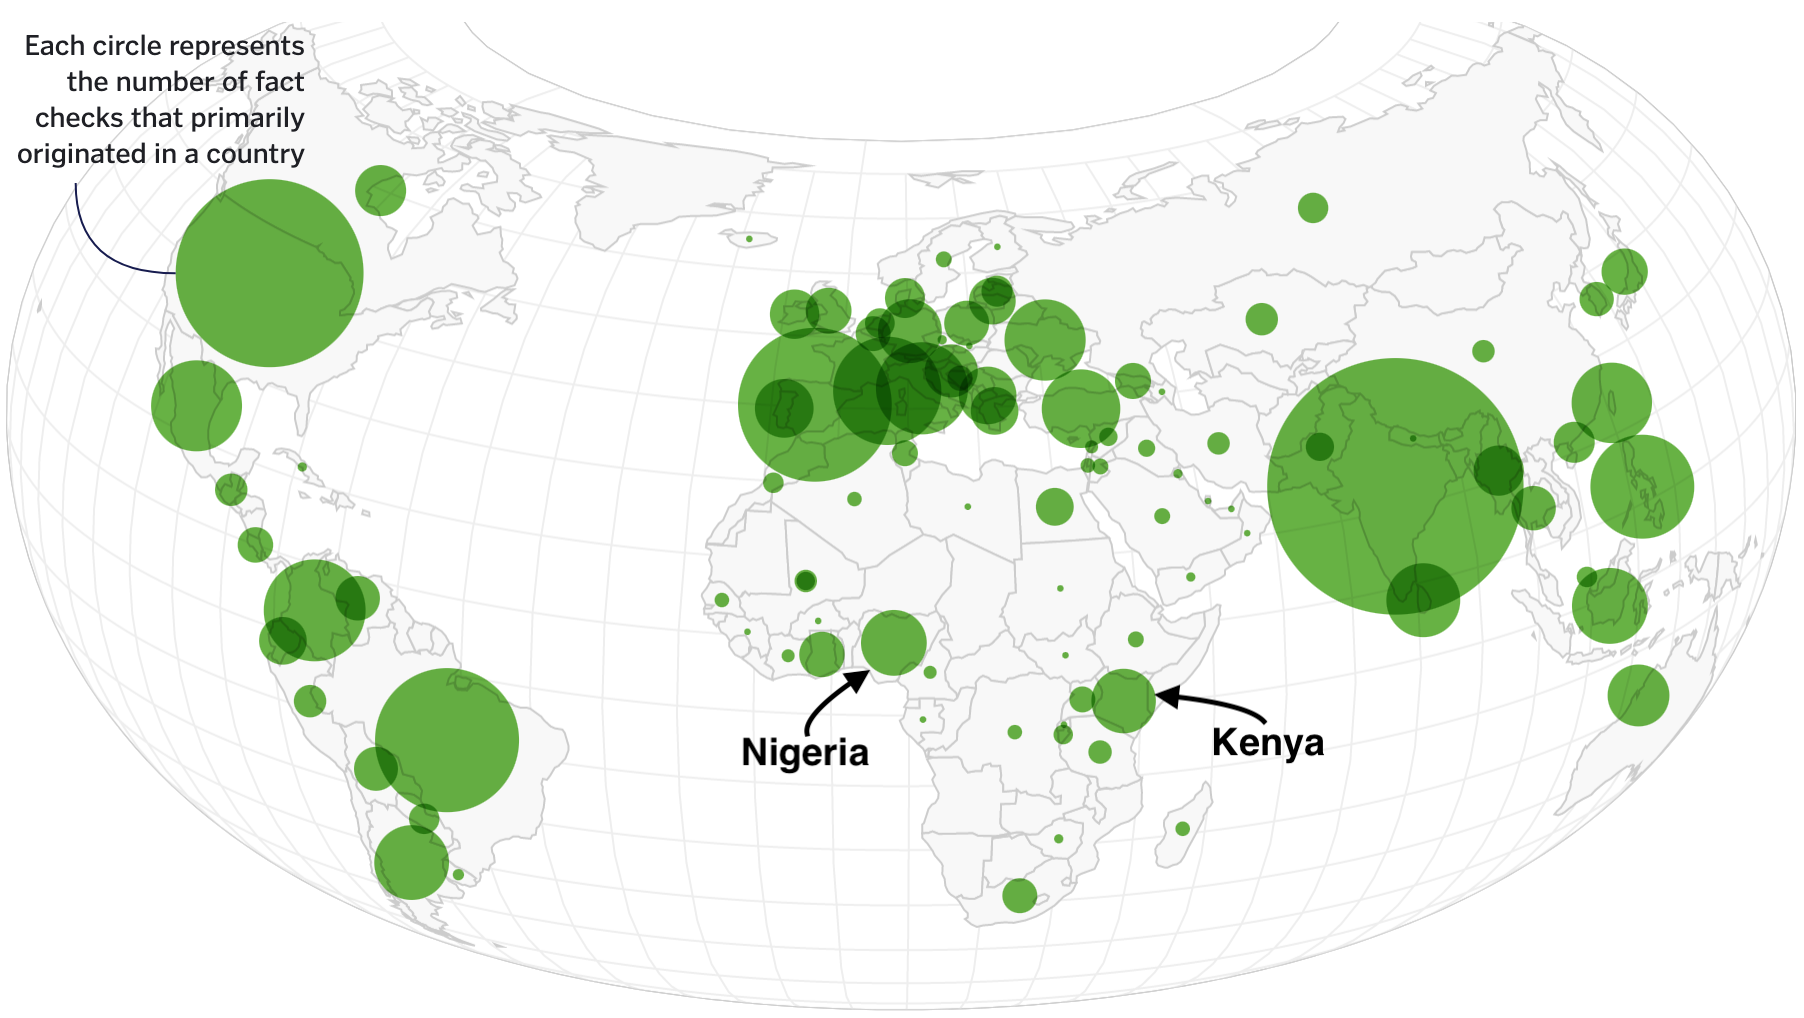
\includegraphics[width=.95\textwidth]{poynter2.png}
\end{figure}


\section{Research Design and Hypotheses}



\subsection{Sample recruitment}
We will recruit respondents in Kenya and Nigeria using Facebook advertisements targeted to users 18 years and older living in these countries.\footnote{Based on previous work it is clear that Facebook imputes location information for some of its users, which can be inaccurate. We will also ask a location screening question to ensure our respondents live in our countries of interest.} To achieve balance on gender within our sample we create separate ads targeting men and women in both countries. Our target sample size is 1,500 respondents in each country for our pilot. Size of the full scale study will be determined following piloting, in procedures described in Section~\textcolor{red}{[TK]}.


Advertisements will appear within Facebook or Instagram, offering users with the opportunity to ``Take a \textcolor{red}{15} minute study about COVID-19 on Messenger'' in exchange for the equivalent of USD \textcolor{red}{0.55} in mobile phone airtime. When users click on the ``Send Message'' button on our advertisement, a Messenger conversation will open with our Facebook page, starting a conversation with a chatbot programmed to implement the survey. In contrast to sending users to an external survey platform such as Qualtrics, the benefit of the chatbot is that we keep users on the Facebook platform, with which they are likely more familiar, and maintain a realistic setting in which users might encounter online misinformation.\footnote{The recruitment advertisement is shown in Figure~\ref{fig:ad} in Appendix~\ref{recruitment}. \color{red}{[[Add images of chatbot once linked to page]]}} Respondents who complete the survey in the chatbot will receive compensation in the form of mobile phone airtime sent to their phone. %%MOW: confirm survey completion time--and update advertisement accordingly

\subsection{Covariates}

We include the below covariates in analysis. The full list of covariates and question wording is in Appendix~\textcolor{red}{[TK]}. \todo{Do we want to do secondary analyses with all covariates? We can conduct this ex-post, we just can't update using the full model. }
\begin{table}[H]
\begin{tabular}{p{0.4\linewidth}p{0.6\linewidth}}
\textbf{Covariate}                   & \textbf{Coded as}                                     \\
\hline
Gender                      & 1   if male, 0 otherwise                     \\
Age                         & Indicators   for population quartiles        \\
Education                                   & Categorical: no/informal schooling, any   primary school, any secondary school, post-seconday qualifications, any   university \\
Religion                    & Categorical: Muslim, Christian, other                     \\
Religiousity                                & Categorical: less than a week, more than once   a week but less than daily, daily                                              \\
No.   people in household   & Indicators   for population quartiles        \\
Index   of scientific views & Indicators for integers 0:2                  \\
Concern regarding COVID-19  & Categorical: ery/somewhat/not worried \\
Perceived government efficacy   on COVID-19 & Categorical:  positive,   neutral, negative                                                                     
\end{tabular}
\end{table}

\todo{Discuss covariates. As is, this is 38,880 unique covariate combinations; is that feasible for implementation with zapier/google sheets/bootstrapping? In practice, make sure we can run this process if we see a category we've never observed before. }
\todo{LR: I think the only one I would think that might not be binary but have a few categories is age (cohorts) and religiosity (frequency of attendance).}

\subsection{Experimental setup}

\subsubsection{Treatment}
Drawing on the literature on experimental interventions to combat misinformation, we include several interventions designed to reduce the spread of misinformation online, which are targeted both at the headline level and respondent level. This list of treatments also draws on real-world interventions that companies and platforms have instituted to combat misinformation. Treatments are presented in Table~\ref{tab:treatments}. 

% interesting point to maybe incorporate: Facebook, 24% of false-rated content in our sample remains up without warning labels \citep{brennen2020types}

\textcolor{red}{[Table to be updated]}
\begin{table}[H]
\begin{tabular}{l|l|l}
\multicolumn{1}{c|}{\textbf{\begin{tabular}[c]{@{}c@{}}Shorthand\\ Name\end{tabular}}} & \multicolumn{1}{c|}{\textbf{\begin{tabular}[c]{@{}c@{}}Treatment\\ Level\end{tabular}}} & \textbf{Treatment}                                                                                                                                                                                                                                                                                                                                                                                              \\ \hline
Facebook tips                                                                                                           & Respondent                                                                                                   &  Facebook's ``Tips to Spot False News'' 
\\
AfricaCheck tips                                                                                                         & Respondent                                                                                                   &  \url{Africacheck.org}'s guide: \\ & & ``How to vet information during a pandemic''                                                                                                                                                                                                                                                                                                                             \\
Video training                                                                                                     & Respondent                                                                                                   &  \href{https://www.bbc.com/news/av/embed/p088bh96/52118949}{BBC Video training}                                                                                                                                                                                                                                                                                                                                                                                  \\
Emotion suppression                                                                                                       & Respondent                                                                                                   & \begin{tabular}[t]{@{}l@{}}Prompt: ``As you view and read the headlines, if you have any \\feelings, please try your best not to let those feelings show.  \\Read all of the headlines carefully, but try to behave so that \\someone watching you would not know that you are feeling\\ anything at all” \citep{gross1998emerging}.\end{tabular}
\\
Accuracy nudge                                                                                 & Respondent                                                                                                   & Placebo headline: ``Do you think this headline accurately\\& & describes an event that actually  happened?'' \\& &  \citep{pennycook2020fighting}.
\\
Deliberation nudge                                                                                 & Respondent                                                                                                   & Placebo headline: ``In a few words, please say \textit{why} you would\\ & & like to share or why you would not like to share this headline.''\\ & & [open text response]
\\
%Context                                                                                                        & Headline                                                                                                     & \begin{tabular}[t]{@{}l@{}}Facebook context button; if you click the info button on an\\ article, a pop-up tells you a few facts about the source: \\ how long the Facebook page has been registered,\\ and has a flag if article is more than 90 days old\end{tabular}
%\\
%Flag                                                                                                           & Headline                                                                                                     &  ``Disputed" flag on the headline                                                                                                                                                                                                                                                                                                                                                     \\
Related articles                                                                                                       & Headline                                                                                                     & Facebook-style related stories: next to story link,\\ & & show one other stories which corrects a false news story                                                                                                                                                                                                                                                                                             \\
Factcheck                                                                                                      & Headline                                                                                                     & Fact checking score by third party\\ & & (e.g., Facebook, AFP, AfricaCheck, etc)
 \\
Control                                                                                                        & N/A                                                                                                          & Control condition                                                                                                                                                                                                                                                                                                                                                                                              
\end{tabular}
\caption{Description of interventions included in the experiment}
\label{tab:treatments}
\end{table}

Respondent-level treatments and headline-level treatments are treated as separate factors, each of which has an empty baseline level that is the control. So respondents may be assigned the pure control condition, one of the respondent-level treatments but no headline-level treatment, one of the headline level treatments but no respondent-level treatment, or one of the respondent-level treatments \textit{and} one of the headline-level treatments. Procedures for calculating treatments assignment probabilities are discussed in section \textcolor{red}{[TK]}. 


\subsubsection{Outcomes and Response Function}

We are interested in decreasing sharing of harmful false information about COVID-19 cures and treatments while not negatively impacting sharing of useful information about transmission and best practices from verified sources. 

\paragraph{Primary Response Function}

We measure interest in sharing information through two questions. The first asks whether the respondent would like to post the article to their Facebook timeline and the second asks whether the respondent would like to send the article to a friend on Facebook. By using a pretest-posttest design \textcolor{red}{[citation]} and an index of repeated measures \citep{broockman2017design}, we aim to improve the efficiency of our design. 

Prior to treatment, we show respondents two articles randomly sourced from our misinformation stimuli and two articles randomly sourced from our true information stimuli, in random order, and for each stimuli we ask the above self-reported interest questions. Respondents are then asked a series of unrelated questions. They are then randomly assigned treatment. If assigned one of the respondent-level treatments, they are administered the relevant treatment. They are then shown two additional misinformation stimuli and two additional true information stimuli, selected from the remaining stimuli that they were \textit{not} shown pre-treatment. If the respondent is assigned a headline-level treatment, this treatment is applied only to the misinformation stimuli, as flags and fact-checking labels are not generally applied to true information from verified sources.\footnote{The initial implementation of Twitter's labeling of coronavirus-related tweets with links to additional information was deemed to be overly broad, and was applied to some tweets that did not include misinformation. Twitter revised their labeling in late June of 2020. A company message was released here on June 26: \url{https://twitter.com/TwitterSupport/status/1276661483561029632}. } For each of the stimuli we again ask the same self-reported interest questions.


We code response to the self-reported interest questions as 1 if the respondent affirms and 0 otherwise. Let $M_i^1$ be the sum of individual $i$'s pre-treatment responses to the \textit{misinformation} stimuli and let $T_i^1$ be the sum of individual $i$'s pre-treatment responses to the \textit{true} informational stimuli. $M_i^2$ and $T_i^2$ are the respective post-treatment responses. Then $M_i^1, T_i^1, M_i^2, T_i^2 \in {0,1,2,3,4}$. 

Our response function is then:
\[
Y_i = -(M_i^2 - M_i^1) + 0.5 \times (T_i^2 - T_i^1)
\]\todo{LR:Made me wonder whether we want to, for power sake, use random effects model w/respondent and headline level REs? so rather than using DV that sums shares across all 4 headlines seen ? This is how psych misinfo studies usually analyze headline-level outcomes and deal with respondent and headline correlations.\\
MOW: Let's discuss, I'm not sure what this would look like for our adaptive agent model. }

Because of random assignment, we expect to see no systematic differences in interest in sharing either true or untrue stimuli across treatment conditions, conditional on covariates. For a given treatment condition, all else equal, if respondents share misinformation at lower rates post-treatment compared to control, this will result in a relatively higher response variable. If respondents share true information at lower rates post-treatment compared to control, this will result in a relatively lower response variable, but the relative impacts are only half as large as those for the misinformation stimuli. 

This response function will be the variable which we optimize for in our adaptive algorithm described in Section~\textcolor{red}{[TK]}, and in our policy learning described in Section~\textcolor{red}{[TK]}. 

\paragraph{Secondary Outcomes}
Additionally, we measure several secondary outcomes, which we will also report. \todo{Formalize how these secondary outcomes are analyzed, based on eventual below linear model.}

These include willingness to read the article, as measured by the question: ``If it were possible, would you click this headline to read the full story?'' As above, we code responses as 1 if the respondent affirms and 0 otherwise. We separately calculate post-treatment minus pre-treatment differences for misinformation and true informational stimuli, and report regressions in the format \textcolor{red}{[TK]}. 

Additionally, we record behavioral measures. At the end of the survey, for each true informational stimuli that the respondent reported they would be interested in sharing, we offer respondents the opportunity to actually share this information as a Facebook post, which has been created on our project Facebook page. We are able to measure whether respondents click on a button which opens a pop-up screen to share the post on Facebook, however, we cannot measure directly whether they then actually follow through to the second step and post the article on their own timeline. Consequently, we report rates of clicking the initial share button in the format \textcolor{red}{[TK]}. Additionally, we report the \textit{aggregate} number of times the associated post for each stimuli was shared. \todo{We \textit{could} actually create a separate post for each treatment combination, and measure sharing that way, but this seems like overkill for a secondary outcome in an already complicated project. } 

And, in order to obtain a behavioral measure of sharing, we collect the articles the respondent indicated they would like to share throughout the survey and at the end of the survey provide links to the \textit{true} information. 

At this point we also debrief respondents, informing them about the headlines they were shown that are false. Instead of allowing respondents to share these headlines, we provide links to tips for spotting misinformation online. 




\section{Data Collection and Design Parameters}

\subsection{Adaptive data collection}
We will collect data using a contextual adaptive experimental design, in which we sequentially update treatment assignment probabilities based on the observed history of treatments, $W_i \in \ww$\footnote{Our treatments is composed of two separate factors, but here we use $W$ to represent combined treatment conditions. Where we wish to explicitly differentiate, we use $W^R_i$ and $W^H_i$ for respondent- and headline-level treatments respectively.}; response,  $Y_i \in \RR$; and covariates, $X_i \in \xx$. Our objective is to learn and evaluate an optimal contextual policy, under which we assign the most effective treatment conditional on covariates. To do this, we use a \textit{contextual bandit} algorithm, which balances \textit{exploration} of the treatment space with \textit{exploitation} of those treatments which we have observed to be effective based on covariates, with batches $b = 1, \dots, B$.  This allows us to continue to learn about treatment effect heterogeneity while improving outcomes over time \textit{within} the frame of the experiment. 

We will use a version of linear Thompson sampling \citep{agrawal2013thompson}. Under Thompson sampling \citep{thompson1933likelihood,thompson1935theory}, treatment is assigned according to the Bayesian posterior probability that each arm is best. In linear Thompson sampling, this is generalized to allow the outcome to be a linear function of covariates. We use a batched approach to updating, collecting data in batches and then updating treatment assignment model after each batch. We discuss size of batches below. 

% \label{subsec:exploration_methods}
Our implementation is based on the balanced linear Thompson sampling method described in \cite{dimakopoulou2017estimation, dimakopoulou2019balanced} :

\begin{enumerate}
\item In the first batch, $b = 1$, we assign treatment uniformly at random. 


\item For batches $b = 2, \dots, B-1$, as determined by the number of batches described in Table~\ref{tab:design}:

\begin{enumerate}
	
 \item Fit a ridge regression model. Use cross-validation to compute the optimal value of the penalization factor $\lambda_{CV}$ using the entire observed history of data.\footnote{For the agent we use a linear model, with treatment indicators, covariates, and treatment and covariates interacted:
 
\begin{align*}
\hat{\mu}_w(X_{i}) & =
			\sum_{w^R} 1\{W^R_i = w^R\}\hat\beta_{w^R}  +
			\sum_{w^H} 1\{W^H_i = w^H\}\hat\beta_{w^H}  +\\ 
			& \sum_{w^R} \sum_{w^H}1\{W^R_i = w^R\} \times 1\{W^H_i =  \hat w^H\}\hat\beta_{w^{R,H}} +  \\
			& \sum_{\ell}  X_{[\ell]i}\hat{\beta}_{\ell} +\\
        &  \sum_{w,\ell} 1\{ W_{i} = w\} X_{[\ell]i} \hat{\beta}_{w, \ell}.
         \label{eq:linear_model_full}
\end{align*} 
The model is estimated using $L_{2}$ penalties for regularization, exclusive of the main treatment effects $\beta_{w^R}$ and $\beta_{w^R}$. Observations are weighted according to stabilized inverse probabilities weights using known assignment probabilities, following \cite{dimakopoulou2017estimation}. Stabilized inverse probability weights are discussed in Appendix~\ref{appendix:stabilized}
}\todo{Have James review model and discuss.}

  \item \label{step:draw} Draw $M$ random samples with replacement from the data, with samples indexed by $m = 1, \dots, M$, so that data from sample $m$ is represented by $D^{(m)} := (X^{(m)}, W^{(m)}, Y^{(m)})$.\footnote{We set M = 100.} 

  \item Within each sample, for each possible context $x$, arm $w$ and bootstrap sample, estimate conditional means  $\hat{\mu}_w^{(m)}(x)$ for each arm using the fitted outcome model. The penalization value is fixed as $\lambda_{CV}$ from step 1, without performing any additional cross-validation.
  
  \item For each context $x$ and available arm $w$, compute and store the following statistics representing the average value of each arm, and the uncertainty associated with this statistic.
    \begin{equation*}
      \begin{aligned}
        \hat{\mu}_w(x)         &= \frac{1}{M}\sum_{m} \hat{\mu}_w^{(m)}(x) \\
         \hat{\sigma}^{2}_w(x) &= \frac{1}{M(M-1)} \sum_{m} (\hat{\mu}_w^{(m)}(x) - \hat{\mu}_w(x))^2
      \end{aligned}
    \end{equation*}

  \item \label{step:prob} Approximate the probability that each arm $w$ is maximal for each possible context $x$. In order to do that, we draw from the following probability distribution a large number $S$ times\footnote{We set S = 1,000.}
  \begin{align*}
    \theta_{w}(x) \sim \mathcal{N}(\hat{\mu}_w(x), \hat{\sigma}_w^{2}(x)) \qquad %\text{for } s \in \{1, \cdots, S\} \text{ and arm }w
    \text{ for all arms }w
  \end{align*}

  and compute the fraction of times that arm $w$ was the largest for each $s$ set of draws
  \begin{align*}
    q_{b}(x, w) = \frac{1}{S} \sum_{s} 1\left\{ \theta_{w}^{(s)}(x) = \max \{\theta_{1}^{(s)}(x), \dots, \theta_{|\mathcal{W}|}^{(s)}(x) \}  \right\}. 
  \end{align*}

  These are the Thompson sampling probabilities associated with the pair $(x, w)$. 
  
  \item Collect data for the batch: For every new subject, collect data on their contexts $x$ and use the probabilities computed in the previous batch to assign arms.
\end{enumerate}

\item For the final batch,  $b = $ B, collect data on-policy:
\begin{enumerate}
  \item Fit a random forest estimator on the entire data set collected through batch $B-1$.
  \item Fit a point-wise optimal policy  by taking the maximum of predicted values for each possible context $x$ 
    \begin{equation*}
     \hat{\pi}_{x} = \arg\max_{ w } \hat{\mu}_{w}(x) . 
    \end{equation*} 
  Store the policy. 
  \item Collect data for the batch: For every new subject, collect data on their contexts, and assign treatment deterministically consistent with $\hat{\pi}_{x}$. 
\end{enumerate}
\end{enumerate}


\subsection{Simulations and design parameters}

\textcolor{red}{[TK]}
\todo{Describe simulation procedures.}

\begin{table}[H]
\centering
\caption{Design parameters} 
\label{tab:design}
\begin{tabular}{l | l}
\textbf{Parameter} & \textbf{Choice set} \\ \hline
First batch size & [100, 200, 400, 800] \\
Number of batches & [3, 4, 5] \\
Total experiment size & [2500, 3750, 5000] \\
%Outcome model & [Ridge, Random Forest] \\
%Balancing weights & [Batch-wise IPW, ARB]\\
Probability floor & [0.01, 0.025, 0.5]\\
\hline
\end{tabular}
\end{table} \todo{Have James review design parameters and discuss.}

\section{Analytic Strategy}

\subsection{Estimating Optimal Policies}



%% below is leftover from the original adaptive preanalysis plan
\section{Policy learning and evaluation}

Following experimental data collection, personalized policies are estimated and evaluated modifying the method explained in \cite{athey2017efficient} and also in \cite{zhou2018offline}; in those approaches, data is collected non-adaptively and is assumed to be iid. In the adaptive setting, we can not make this assumption about the data. Instead, the sample is split into an initial training period on which we learn the optimal policy using the adaptive agent, and a period of on-policy evaluation. 


%% rather than it's own section we could also integrate hypotheses into the next section (analytic strategy)--e.g. say how we will analyze results and what we expect
\subsection{Hypotheses}


\subsubsection{Optimal interventions:}

Our primary hypotheses of interest relate the value of an estimated optimal contextual policy $\pi_{opt}$ to fixed policies $\pi_{W}$ and the value of fixed policies $\pi_{W}$ to control $\pi_{CTR}$.

\todo{Update hypotheses}

\begin{enumerate}
\item[ ] 
We determine whether any of the treatments improve over the control. 
\begin{hypothesis} The best fixed policy ($\pi_{w_{\textrm{max} } }$) achieves higher value than the control policy ($\pi_{CTR}$)   \label{eq:control_null}
\begin{align*}
H_{0}: Q(\pi_{w_{\textrm{max} } }) = Q(\pi_{CTR}) \qquad H_{a}:  Q(\pi_{w_{\textrm{max} } }) > Q(\pi_{CTR})
\end{align*}
\end{hypothesis}
  \item[ ]
  
  Analyzing heterogeneity in treatment effects allows us to learn whether different interventions are more effective for different people, improving our understanding of how to tackle harmful misinformation during an ongoing health crisis.
  \begin{hypothesis}
  The best contextual policy that can be estimated from the data ($\pi_{opt}$) achieves higher value than the best fixed policy ($\pi_{w_{\textrm{max} } }$)\label{eq:bestfix_null}
\begin{align*}
  H_{0}: Q(\pi_{opt}) = Q(\pi_{w_{\textrm{max}}}) \qquad H_{a}:  Q(\pi_{opt}) > Q(\pi_{w_{\textrm{max}}})
\end{align*}
\end{hypothesis}
\end{enumerate}



We then estimate the value of the policy on the remaining observations. To evaluate the policies, take the average scores :
    \begin{align*}
          \widehat{Q}({\pi}_{w})  &:= \frac{1}{\bigg{\lvert} \bigcup\limits_{b=1}^{B-1} \mathcal{I}_{b} \bigg{\rvert}} \sum_{t \in \bigcup\limits_{b=1}^{B-1} \mathcal{I}_{b} } \widehat{\Gamma}_{w,t} \quad \text{for fixed policies $w$}\\
                     \widehat{Q}(\hat{\pi}_{opt})  &:= \frac{1}{\big{\lvert}  \mathcal{I}_{B} \big{\rvert}} \sum_{t \in \mathcal{I}_{B} }
                      \langle \hat{\pi}_{t}, \widehat{\Gamma}_{\cdot, t}  \rangle 
    \end{align*}




\textcolor{red}{LR: Secondary hypotheses: Do we want to specify that among the control group we will analyze the predictors of willingness to share fake news (maybe in this case more than true info, bc we want to predict ppl most susceptible to sharing falsities rather than just "always sharers")? -- some thing we might hypothesize: belief in science/religiosity/COVID knowledge will be negatively correlated with sharing false cures... Age/trust in media will be positively correlated with sharing false cures. gender? [I dont have strong priors]. Unlike the US I think there will NOT be a strong correlation btw partisanship and willingness to share cures.\\
MOW: I don't really have a position on this...happy to include if we think it is of interest.}





\clearpage
\bibliographystyle{apalike}
\bibliography{fb_misinfo_references}

\clearpage
\appendix

\section{Recruitment}\label{recruitment}

\begin{figure}[htb]
\centering
\caption{Advertisement as run in Facebook timeline.}
\label{fig:ad}
\includegraphics[width=.5\textwidth]{../irb/recruitment_advert.png}
\end{figure}


\section{Matrix method, outcome model, and balancing weights}
\subsection{Matrix method} 
To estimate the value of a given policy, we may use an outcome model, weights, or both. Here, the estimated counterfactual rewards, $\{\hat{\Gamma}_{i,k}\}_{k=1}^{|\mathcal{W}|}$, may be estimated via,
\begin{itemize}
\item \textbf{Inverse probability weighted estimation}, using a version of Horvitz-Thompson estimator \citep{horvitz1952}
\begin{align}
\hat{\Gamma}_w^{HT} & =  \frac{1}{n} \sum_{i = 1}^n 1 \{ W_i = w\} \gamma_i Y_i. 
\end{align}
\item \textbf{Adaptively weighted doubly-robust estimation}. 
\label{appendix:doubly-robust}
\textcolor{red}{[To be further filled in, with reference to LFO paper.]}\\
We estimate an $n \times |\mathcal{W}|$ matrix of \textit{doubly-robust scores} $\hat{\Gamma}_{i,w}$. For each treatment $w$ and observation $i$, we compute    
      \begin{align}
        \hat{\Gamma}_{i,w} = \hat{\mu}_{w}(X_{i}) + 1 \{W_i = w \} \gamma_{i}(Y_{i} - \hat{\mu}_w(X_i))
    \end{align}
  The term involving the balancing weights, $\gamma_i$, is a correction that mitigates selection bias arising from not collecting the data by assigning treatments uniformly at random; we use stabilized inverse probabilities weights described below. Each element of this matrix is a (corrected) estimate of the average reward that the observation $i$ would have received had they been given treatment $w$.
\end{itemize}


\subsubsection{Batch-wise stabilized inverse probability weighting} \label{appendix:stabilized}
Instead of using the raw inverse probability weights, we normalize the weights to one, which can improve mean squared error of the associated estimator. 

\begin{align}
\left.
\gamma^{SIPW}(x, w, b) = \frac{ 1 }{e_{w}^{\pi^{(b)}}(x)}   
\middle/ 
{ \sum_{j = 1}^T \frac{1\{W_{j} = w\}}{e_{w}^{\pi^{(B_j)}}(X_i)} }
\right.
\end{align}

\todo{Add survey instrument}

\end{document}